\section{Installation, Example Usage and Tutorial} \label{examples}

In this section, we illustrate the main functionality and scope of \means{}  in the form of a user tutorial.
The tutorial instructions below are auto-generated from the interactive tutorial in the IPython notebook format (\autoref{fig:screenshot:tutorial:simulation}).

\begin{figure}[ht]
    \centering
    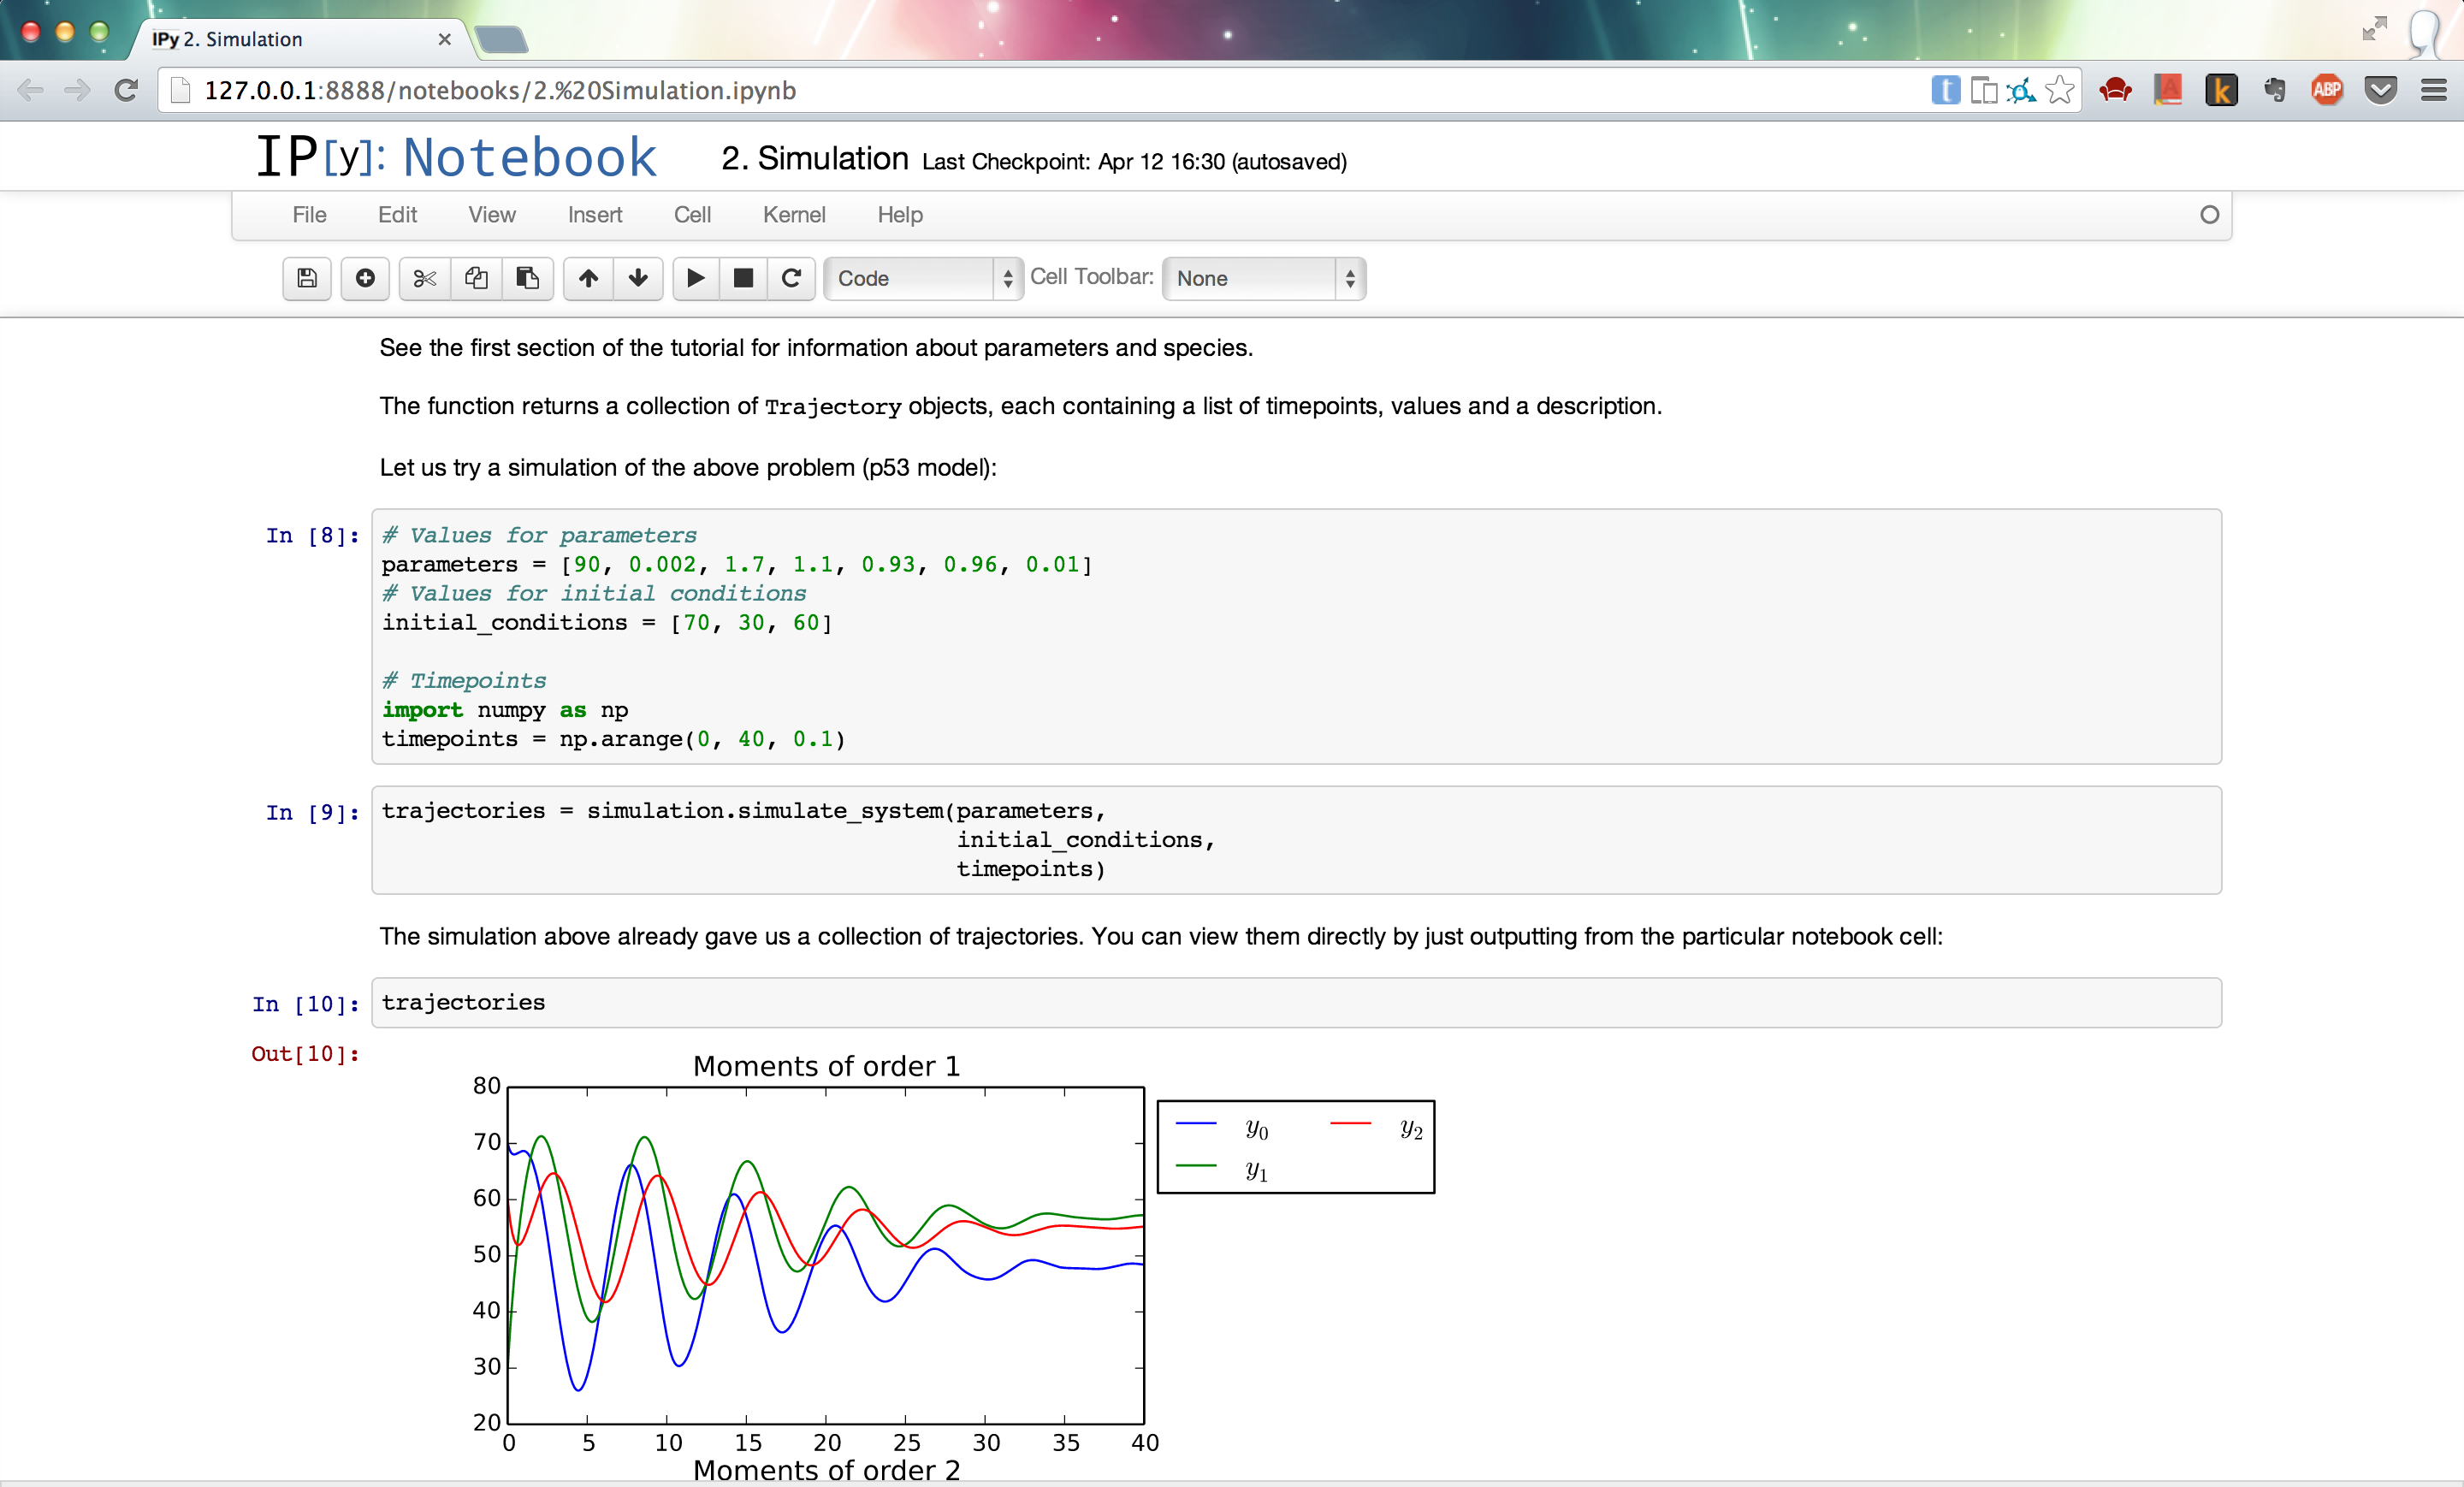
\includegraphics[width=0.9\textwidth]{handmade_figures/tutorial-screenshot.png}
    \caption{A screenshot of the IPython notebook running the Simulation section of the tutorial (\autoref{sec:simulation} of this document).}
    \label{fig:screenshot:tutorial:simulation}
\end{figure}

Even though have tried our best to integrate the tutorial this document nicely, paper 
might not be the best medium for this content. 
Therefore, for the convenience of the reader, we also provide online read-only version of this tutorial, available at \url{http://msc.bc.ic.ac.uk:2712/}. 

If the reader has access to a working \means{} and \verb"IPython" installation together with \means{} source-code,
aforementioned fully operational interactive version of the tutorials could be run directly in the IPython notebook by typing:

\begin{InputVerbatim}
cd examples/Tutorials
ipython notebook
\end{InputVerbatim}

A new browser window with the interactive tutorial should pop up seconds after inputting this command.

\subsection{Installation}

In order to install \means{} package, one must first make sure all external dependancies such as \verb"sundials" libraries \cite{hindmarsh_sundials_2005} are installed. 
Our \verb"README.txt" file located in the \verb"src" directory of the codebase provides some guidance on how to do this.

Once the dependancies are all accounted for, the development version of the \means{} package can be installed by navigating to the \verb"src" directory of the codebase, and issuing the install command via a standard \py{} package installation tool \verb"pip":

\begin{InputVerbatim}
pip install -e .
\end{InputVerbatim}

This command should fetch and install all the dependancies of \means{} as well as the package in the development mode (specified by the \verb"-e" flag). 
Troubleshooting information is provided in the same \verb"README.txt" file.

Note that in order to be able to use the \means{} package to its full potential, the user is encouraged to install the latest version of  IPython notebook\cite{perez_ipython:_2007} as well.

Once the code is released to public, \means{} could be immediately pushed to \gls{pypi}, what would allow to shorten the installation procedure to just \verb"pip install means" command.

{   % These brackets are very important, btw.

    % IPython notebook likes to define their own colours...
    % And who could blame them.
    
    \definecolor{orange}{cmyk}{0,0.4,0.8,0.2}
    \definecolor{darkorange}{rgb}{.71,0.21,0.01}
    \definecolor{darkgreen}{rgb}{.12,.54,.11}
    \definecolor{myteal}{rgb}{.26, .44, .56}
    \definecolor{gray}{gray}{0.45}
    \definecolor{lightgray}{gray}{.95}
    \definecolor{mediumgray}{gray}{.8}
    \definecolor{inputbackground}{rgb}{.95, .95, .85}
    \definecolor{outputbackground}{rgb}{.95, .95, .95}
    \definecolor{traceback}{rgb}{1, .95, .95}
    % ansi colors
    \definecolor{red}{rgb}{.6,0,0}
    \definecolor{green}{rgb}{0,.65,0}
    \definecolor{brown}{rgb}{0.6,0.6,0}
    \definecolor{blue}{rgb}{0,.145,.698}
    \definecolor{purple}{rgb}{.698,.145,.698}
    \definecolor{cyan}{rgb}{0,.698,.698}
    \definecolor{lightgray}{gray}{0.5}
    
    % bright ansi colors
    \definecolor{darkgray}{gray}{0.25}
    \definecolor{lightred}{rgb}{1.0,0.39,0.28}
    \definecolor{lightgreen}{rgb}{0.48,0.99,0.0}
    \definecolor{lightblue}{rgb}{0.53,0.81,0.92}
    \definecolor{lightpurple}{rgb}{0.87,0.63,0.87}
    \definecolor{lightcyan}{rgb}{0.5,1.0,0.83}
    
    % Tutorials go here
    \input{autogenerated-tutorials}
}   % make sure to put them above this line

